\section{Conditional convergence to De Giorgi's mean curvature flow}

In this section, we shall state our solution concept and prove convergence to 
the aforementioned.

\subsection{Definition of $ \bv $-solutions to De Giorgi's mean curvature flow}

\begin{definition}[$\bv$-solution to  De Giorgi's multiphase mean curvature 
flow]
	\label{de_giorgi_solution_to_mmcf}
	Fix some finite time horizon $ T < \infty $, a $ P \times P $ matrix of 
	surface tensions $ \sigma $ and initial data $ \chi^{ 0 } \colon \flattorus 
	\to \{ 0 , 1 \}^{ P } $ with $ \energy_{ 0 } \coloneqq ( \chi^{ 0 } ) $ and 
	$ \sum_{ i = 1 }^{ P } \chi_{ i }^{ 0 } = 1 $. We say that
	\begin{equation*}
		\chi \in \cont \left(
		[ 0 , T ]
		;
		\lp^{ 2 } \left( \flattorus ; \{ 0 , 1 \}^{ P } \right)
		\right)
	\end{equation*}
	with $ \esssup_{ 0 \leq t \leq T } \energy ( \chi ) $ and $ \sum_{ i = 1 
	}^{ P } \chi_{ i } = \sum_{ i = 1 }^{ P } \mathds{ 1 }_{ \Omega_{ i } } = 
	1  $ \emph{is a } $\bv$-\emph{solution to De Giorgi's mean 
	curvature flow with initial data} $ \chi^{ 0 } $ \emph{and surface 
	tensions} $ \sigma $ if the following holds. 
	\begin{enumerate}
		\item 
		For all $ 1 \leq i \leq P $, there exist normal 
		velocities $ V_{ i } \in \lp^{ 2 } ( \abs{ \nabla \chi_{ i } } \dd{ t } 
		) $ 
		of the interfaces 
		in the sense that
		\begin{equation*}
			\partial_{ t } \chi_{ i }
			=
			V_{ i } \abs{ \nabla \chi_{ i } } \dd{ t }
		\end{equation*}
		holds in the distributional sense on $ ( 0 , T ) \times \flattorus $.
		
		\item 
		There exist a mean curvature vector $ H \in 
		\lp^{ 2 } ( \energy ( u ; \cdot) \dd{ t } ; \mathbb{ R }^{ d } ) $ 
		which satisfies
		\begin{equation*}
			\sigma_{ i j }
			\int_{ 0 }^{ T }
				\energy \left( \chi ; \inner*{ H }{ \xi } \right)
			\dd{ t }
			=
			-
			\sum_{ 1 \leq i < j \leq P }
			\sigma_{ i j }
			\int_{ 0 }^{ T }
				\int_{ \Sigma_{ i , j } }
					\inner*{
						\diff \xi }
					{ \mathrm{Id} - \nu_{ i } \otimes \nu_{ i } }
				\dd{ \hm^{ d - 1 } }
			\dd{ t }
		\end{equation*}
		for all test vector fields 
		$ \xi \in \cont_{ \mathrm{c} }^{ \infty } \left(
			( 0 , T ) \times \flattorus ; \mathbb{ R }^{ d }
		\right) $,
		where $ \nu_{ i } \coloneqq \nabla \chi_{ i } / \abs{ \nabla \chi_{ i } 
		} $ are the inner unit normals and $ \Sigma_{ i , j } \coloneqq 
		\partial_{ \ast } \Omega_{ i } \cap \partial_{ \ast } \Omega_{ j } $
		is the $ (i, j )$-th interface.
		
		\item 
		The partition $ \chi $ satisfies a De Giorgi type optimal energy 
		dissipation inequality in the sense that for almost every time $ 0 < T' 
		< T $, we have
		\begin{equation*}
			\energy ( \chi ( T' ) )
			+
			\frac{ 1 }{ 2 }
			\sum_{ 1 \leq i < j \leq P }
				\sigma_{ i , j }
				\int_{ 0 }^{ T' }
					\int_{ \Sigma_{ i , j } }
						V_{ i }^{ 2 }
						+
						H^{ 2 }
					\dd{ \hm^{ d - 1 } }
				\dd{ t }
			\leq
			\energy ( \chi^{ 0 } ).
		\end{equation*}
		
		\item
		The initial data is achieved in the space $ \cont \left( [ 0 , T ] ; 
		\lp^{ 2 } ( \flattorus ) \right) $.
	\end{enumerate}
\end{definition}

\begin{theorem}
	\label{convergence_to_de_giorgis_multiphase_mcf}
	Let a smooth multiwell potential $ W \colon \mathbb{ R }^{ N } \to [ 0, 
	\infty ) $ satisfy the assumptions 
	(\ref{polynomial_growth})-(\ref{perturbation bound}). Let $ T < \infty 
	$ be an arbitrary finite time horizon. Given a sequence of initial data 
	$ u_{ \varepsilon }^{ 0 } \colon \flattorus \to \mathbb{ R }^{ N } $ 
	approximating a partition 
	$ \chi^{ 0 } \in \bv \left( \flattorus ; \{ 0 , 1 \}^{ P } \right) $ 
	in the sense that 
	$ u_{ \varepsilon }^{ 0 } \to u^{ 0 } =  \sum_{ 1 \leq i \leq P } 
	\chi_{ i }^{ 0 } \alpha_{ i } $ 
	holds pointwise almost everywhere and 
	\begin{equation*} 
		\energy_{ 0 } 
		\coloneqq 
		\energy ( \chi^{ 0 } ) 
		= 
		\lim_{ \varepsilon \to 0 } 
		\energy_{ \varepsilon } ( u_{ \varepsilon }^{ 0 } ) 
		< 
		\infty,
	\end{equation*}
	we have that for 
	some subsequence of solutions to the Allen--Cahn equation
	(\ref{allen_cahn_eq}) $ u_{\varepsilon } $ with initial datum $ u_{ 
		\varepsilon }^{ 0 } $, there exists a time-dependent partition $ \chi $ 
	with 
	$ \chi \in \bv \left( ( 0 , T ) \times \flattorus ; \{ 0 , 1 \}^{ P } 
	\right) $ and
	$ \chi 
	\in \cont \left( [ 0 , T ] ; \lp^{ 2 } \left( \flattorus ;  \{ 0 , 1 
	\}^{ P } \right) \right) $ such that $ u_{ \varepsilon } $ converges to 
	$ u \coloneqq \sum_{ 1 \leq i \leq P } \chi_{ i } \alpha_{ i } $ almost 
	everyhwere. Moreover $ u $ assumes the initial data $ u^{ 0 } $ in $ 
	\cont \left( [ 0, T ] ; \lp^{ 2 }( \flattorus ) \right) $. If we 
	additionally assume that the 
	time-integrated energies converge (\ref{energy_convergence}), then $ 
	\chi $ is a $ \bv $-solution to De Giorgis mean curvature flow in the sense 
	of 
	\Cref{de_giorgi_solution_to_mmcf}.
\end{theorem} 

This result is similar to \Cref{convergence_to_multiphase_mcf} and we only need 
to prove that $ \chi $ is a $ \bv $-solution to De Giorgis mean curvature flow.

\begin{proof}
	Let us for simplicity first consider the twophase case. The idea of the 
	proof is that we already have an optimal energy dissipation inequality for 
	the Allen--Cahn equation given by (\ref{energy_dissipation_sharp}).
	If we use that additionally use the Allen--Cahn equation once, we arrive at 
	the reformulated version of the optimal energy dissipation inequality given 
	by
	\begin{equation*}
	\label{energy_dissipation_sharp_with_curvature}
	\energy_{ \varepsilon } ( u_{ \varepsilon } ( T' ) )
	+
	\frac{ 1 }{ 2 }
	\int_{ 0 }^{ T' }
		\int
			\varepsilon \abs{ \partial_{ t } u_{ \varepsilon } }^{ 2 }
			+
			\frac{ 1 }{ \varepsilon }
			\abs{
				\varepsilon \Delta u_{ \varepsilon } 
				-
				\frac{ 1 }{ \varepsilon } \nabla W ( u_{ \varepsilon } )
			}^{ 2 }
		\dd{ x }
	\dd{ t }
	\leq
	\energy_{ \varepsilon } ( u_{ \varepsilon}^{ 0 } ).
	\end{equation*}
	Our hope is that as $ \varepsilon $ tends to zero, we can pass to the 
	optimal energy dissipation inequality for $ \chi $ through lower 
	semicontinuity. 
	Since we assume the convergence of the inital energies and energy 
	convergence for almost every time, the only terms we have to care about are 
	the lower semicontinuity of the velocity term, which reads
	\begin{equation}
		\label{lsc_of_velocity}
		\liminf_{ \varepsilon \to 0 }
			\frac{ 1 }{ 2 }
			\int_{ 0 }^{ T' }
				\int
					\varepsilon 
					\abs{ \partial_{ t } }^{ 2 }
				\dd{ x }
			\dd{ t }
		\geq
		\frac{ 1 }{ 2 }
		\sum_{ 1 \leq i < j \leq P }
			\sigma_{ i , j }
			\int_{ 0 }^{ T' }
				\int_{ \Sigma_{ i , j } }
					V_{ i }^{ 2 }
				\dd{ \hm^{ d - 1 } }
			\dd{ t },
	\end{equation}
	and the lower semicontinuity of the curvature term, which reads
	\begin{equation}
		\label{lsc_of_curvature}
		\liminf_{ \varepsilon \to 0 }
			\frac{ 1 }{ 2 }
			\int_{ 0 }^{ T' }
				\int
					\frac{ 1 }{ \varepsilon }
					\abs{
						\varepsilon
						\Delta u_{ \varepsilon }
						-
						\frac{ 1 }{ \varepsilon }
						\nabla W ( u_{ \varepsilon } ) 
					}^{ 2 }
				\dd{ x }
			\dd{ t }
		\geq
		\frac{ 1 }{ 2 }
		\sum_{ 1 \leq i < j \leq P }
			\sigma_{ i , j }
			\int_{ 0 }^{ T' }
				\int_{ \Sigma_{ i , j } }
					H^{ 2 }
				\dd{ \hm^{ d - 1 } }
			\dd{ t }.
	\end{equation}
	Moreover we have to show existence of the mean curvature function $ H $.
	We could cheat in this step and simply use that by 
	\Cref{convergence_to_multiphase_mcf}, we already know that the tangential 
	convergence applied to $ \xi $ is given by the velocity, or in other words, 
	that we already have $ V_{ i } = H $ on $ \Sigma_{ i , j } $. But we want 
	to present a more direct approach.
	
	Consider the linear functional 
	\begin{equation*}
		L ( \xi )
		\coloneqq
		- \sum_{ 1 \leq i < j \leq P }
			\sigma_{ i j }
			\int_{ 0 }^{ T }
				\int_{ \Sigma_{ i j } }
					\inner*{ \diff \xi }{ \mathrm{Id} - \nu_{ i } \otimes \nu_{ 
					i } }
				\dd{ \hm^{ d - 1 } }
			\dd{ t }
	\end{equation*}
	defined on test vector fields $ \xi $. Then $ L $ is bounded with respect 
	to $ \lp^{ 2 } \left( ( 0 , T ) \times \flattorus ; \mathbb{ R }^{ d } ; 
	\energy ( \xi ; \cdot ) \right) $ since by the convergence of the curvature 
	term observed in $ \Cref{convergence_of_curvature_multiphase} $, we have
	\begin{align*}
		\abs{ L ( \xi ) }
		& =
		\liminf_{ \varepsilon \to 0 }
			\abs{ 
				-
				\int_{ 0 }^{ T }
					\int
						\inner*{
							\varepsilon \Delta u_{ \varepsilon } 
							-
							\frac{ 1 }{ \varepsilon }
							\nabla W ( u_{ \varepsilon } )
						}
						{ \diff u_{ \varepsilon } \xi }
					\dd{ x }
				\dd{ t }
			}
		\\
		& \leq
		\left(
			\int_{ 0 }^{ T }
				\int
					\frac{ 1 }{ \varepsilon }
					\abs{ 
						\varepsilon \Delta u_{ \varepsilon }
						-
						\frac{ 1 }{ \varepsilon }
						\nabla W ( u_{ \varepsilon } )
					}^{ 2 }
				\dd{ x }
			\dd{ t }
		\right)^{ 1/2 }
		\left(
			\int_{ 0 }^{ T }
				\int
					\varepsilon
					\abs{ \nabla u_{ \varepsilon } }^{ 2 }
					\abs{ \xi }^{ 2 }
				\dd{ x }
			\dd{ t }
		\right)^{ 1/2 }
		\\
		& \leq
				\left(
		\int_{ 0 }^{ T }
		\int
		 \varepsilon
		\abs{ 
		\partial_{ t } u_{ \varepsilon }
		}^{ 2 }
		\dd{ x }
		\dd{ t }
		\right)^{ 1/2 }
		\left(
		\int_{ 0 }^{ T }
		\int
		\varepsilon
		\abs{ \nabla u_{ \varepsilon } }^{ 2 }
		\abs{ \xi }^{ 2 }
		\dd{ x }
		\dd{ t }
		\right)^{ 1/2 }.
	\end{align*}
	The first factor stays uniformly bounded due to the energy dissipation 
	inequality (\ref{energy_dissipation_sharp}), and by the equipartition of 
	energies (\Cref{equipartition_of_energies_multiphase}), the second factor 
	converges to the $ \lp^{ 2 } $-norm if $ \xi $ with respect to the energy 
	measure, proving our claim. But therefore we can extend the functional to 
	the square integrable functions with respect to the energy measure, and by 
	Riesz representation theorem obtain the existence of the desired mean 
	curvature vector $ H $.
	
	Let us moreover firstly consider the lower semicontinuity of the curvature 
	term. Let again $ \xi $ be some test vector field. Then for all $ 
	\varepsilon > 0 $ and some fixed time, we have by Young's inequality and 
	Cauchy--Schwarz that
	\begin{align*}
		& 
		\liminf_{ \varepsilon \to 0 }
		\frac{ 1 }{ 2 }
		\int
			\frac{ 1 }{ \varepsilon }
			\abs{ 
				\varepsilon
				\Delta u_{ \varepsilon }
				-
				\frac{ 1 }{ \varepsilon }
				\nabla W ( u_{ \varepsilon } )
			}^{ 2 }
		\dd{ x }
		\\
		\geq{} &
		\liminf_{ \varepsilon \to 0 }
		\int
			\inner*{ 
				\varepsilon
				\Delta u_{ \varepsilon }
				-
				\frac{ 1 }{ \varepsilon }
				\nabla W ( u_{ \varepsilon } )
			}{
				\diff u_{ \varepsilon } \xi
			}
		\dd{ x }
		-
		\frac{ 1 }{ 2 }
		\int 
			\varepsilon
			\abs{ \nabla u_{ \varepsilon } }^{ 2 }
			\abs{ \xi }^{ 2 }
		\dd{ x }
		\\
		={} &
		-\energy \left( \chi ; \inner*{ H }{ \xi } \right)
		-
		\frac{ 1 }{ 2 }
		\energy \left( \chi ; \abs{ \xi }^{ 2 } \right).
	\end{align*}
	Since this inequality holds for any test vector field, we may take a 
	sequence of test vector fields satisfying
	\begin{equation*}
		\lim_{ n \to \infty }
			\norm{ \xi_{ n } + H }_{ \lp^{ 2 } \left( \flattorus ; \energy 
			( 
			\chi ; \cdot ) \right) } 
		=
		0.
	\end{equation*}
	This then yields the desired inequality (\ref{lsc_of_curvature}) by 
	applying Fatou's Lemma to pull the limes inferior into the time integral.
	
	In principle the proof is now already done, since 
	\Cref{convergence_to_multiphase_mcf} already gives us that for almost every 
	time $ t $, we already have $ V_{ i } \nu_{ i } = - H $ on $ \Sigma_{ i , j 
	} $ $ \hm^{ d-  1 } $-almost everyhwere. But since this makes heavy use of 
	the previous arguments, we instead want to present another proof which 
	directly proves the lower semicontinuity of the velocity term.
	
	Let us first consider the 
	scalar case $ N = 1 , P = 2 $. By a similar duality argument as for the 
	lower semicontinuity of the curvature term, we compute 
	that for 
	every test function $ \varphi $, we have
	\begin{align*}
		& \liminf_{ \varepsilon \to 0 }
			\frac{ 1 }{ 2 }
			\int_{ 0 }^{ T }
				\int
					\varepsilon \abs{ \partial_{ t } u_{ \varepsilon } }^{ 2 }
				\dd{ x }
			\dd{ t }
		\\
		\geq{} &
		\liminf_{ \varepsilon \to 0 }
			\int_{ 0 }^{ T }
				\int
					\partial_{ t } u_{ \varepsilon } 
					\phi ' ( u_{ \varepsilon } )
					\varphi
				\dd{ x }
			\dd{ t }
		-
		\frac{ 1 }{ 2 }
		\int_{ 0 }^{ T }
			\int
				\frac{ 1 }{ \varepsilon }
				\left( \phi ' ( u_{ \varepsilon } ) \varphi \right)^{ 2 }
			\dd{ x }
		\dd{ t }
		\\
		\geq{} &
		\liminf_{ \varepsilon \to 0 }
			\int_{ 0 }^{ T }
				\int
					\partial_{ t } \psi
					\varphi
				\dd{ x }
			\dd{ t }
			-
			\frac{ 1 }{ 2 }
			\int_{ 0 }^{ T }
				\int
					\frac{ 1 }{ \varepsilon }
					2 W ( u_{ \varepsilon } )
					\varphi^{ 2 }
				\dd{ x }
			\dd{ t }
		\\
		={} &
		\sigma
		\int_{ 0 }^{ T }
			\int_{ \Sigma }
				\varphi V
			\dd{ \hm^{ d - 1 } }
		\dd{ t }
		-
		\frac{ 1 }{ 2 }
		\sigma
		\int_{ 0 }^{ T }
			\int_{ \Sigma }
				\varphi^{ 2 }
			\dd{ \hm^{ d - 1 } }
		\dd{ t }.
	\end{align*}	
	Since again the inequality holds for any testfunction $ \varphi $, we may 
	plug in a sequence of testfunctions $ \varphi_{ n } $ satisfying
	\begin{equation*}
		\lim_{ n \to \infty }
			\norm{ \varphi_{ n } - V }_{ \lp^{ 2 } \left( ( 0 , T ) \times 
			\flattorus ; \dd{ \hm^{ d - 1 } } |_{ \Sigma } \dd{ t } \right) }
		= 0
	\end{equation*}
	and thereby obtain the desired inequality (\ref{lsc_of_velocity}).
	
	For the multiphase case, we do not find an immediate generalization of this 
	proof, but rather have to work with the usual localization argument to 
	obtain a reduction to the scalar case.
	
	As in the proof of \Cref{convergence_to_multiphase_mcf}, let $ \delta > 0 $ 
	and $ 0 = T_{ 0 } < T_{ 1 } < \dotsc < T_{ K } = T' $ be a partition of $ [ 
	0 , T' ] $. Let $ ( g_{ k } )_{ k = 1 , \dotsc , K } $ be a partition of 
	unity with respect to the intervals $ ( T_{ 0 } - \delta , T_{ 1 } + \delta 
	), \dotsc , ( T_{ K - 1 } - \delta , T_{ K } + \delta ) $ and let $ r > 0 
	$, where $ \eta_{ B } $ and $ \rho_{ B } $ are as in 
	\Cref{localization_lemma_with_normals}. Then we estimate
	\begin{align*}
		 A \coloneqq{}& \liminf_{ \varepsilon \to 0 }
			\frac{ 1 }{ 2 }
			\int_{ 0 }^{ T }
				\int
					\varepsilon
					\abs{ \partial_{ t } u_{ \varepsilon } }^{ 2 }
				\dd{ x }
			\dd{ t }
		\\
		={} &
		\liminf_{ \varepsilon \to 0 }
			\sum_{ k = 1 }^{ K }
				\sum_{ B \in \mathcal{ B }_{ r } } 
					\frac{ 1 }{ 2 }
					\int_{ 0 }^{ T }
						\int
							g_{ k } \eta_{ B }
							\varepsilon
							\abs{ \partial_{ t } u_{ \varepsilon } }^{ 2 }
						\dd{ x }
					\dd{ t }
		\\
		\geq{} &
		\liminf_{ \varepsilon \to 0 }
			\sum_{ k = 1 }^{ K }
				\sum_{ B \in \mathcal{ B }_{ r } }
					\max_{ 1 \leq i \leq P }
						\sup_{ 
							\substack{ 
								\varphi \in \cont_{ \mathrm{c} }^{ \infty } 
								\left( ( 0 , T ) \times \flattorus \right)
								\\
								\abs{ \varphi } \leq R  
							}
						}
							\int_{ 0 }^{ T }
								\int
									g_{ k } \eta_{ B }
									\inner*{ \nabla \phi_{ i } ( u_{ 
									\varepsilon 
									} ) }{ \partial_{ t } u_{ \varepsilon } }
									\varphi
								\dd{ x }
							\dd{ t } 
		\\
							& \qquad \qquad \qquad \qquad \qquad \qquad \quad 
							\:\, -
							\frac{ 1 }{ 2 }
							\int_{ 0 }^{ T }
								\int
									g_{ k } \eta_{ B }
									\frac{ 1 }{ \varepsilon }
									\abs{ \nabla \phi_{ i } ( u_{ \varepsilon } 
									) }^{ 2 }
									\varphi^{ 2 }
								\dd{ x }
							\dd{ t }
		\\
		\geq{} &
		\liminf_{ \varepsilon \to 0 }
		\sum_{ k = 1 }^{ K }
		\sum_{ B \in \mathcal{ B }_{ r } }
		\max_{ 1 \leq i \leq P }
		\sup_{ 
			\substack{ 
				\varphi \in \cont_{ \mathrm{c} }^{ \infty } 
				\left( ( 0 , T ) \times \flattorus \right)
				\\
				\abs{ \varphi } \leq R  
			}
		}
		\int_{ 0 }^{ T }
		\int
		g_{ k } \eta_{ B }
		\partial_{ t } \psi_{ i }^{ \varepsilon }
		\varphi
		\dd{ x }
		\dd{ t } 
		\\
		& \qquad \qquad \qquad \qquad \qquad \qquad \quad 
		\:\, -
		\frac{ 1 }{ 2 }
		\int_{ 0 }^{ T }
		\int
		g_{ k } \eta_{ B }
		\frac{ 1 }{ \varepsilon }
		2 W ( u_{ \varepsilon } )
		\varphi^{ 2 }
		\dd{ x }
		\dd{ t }
	\end{align*}
	Pulling the limes inferior inside the double sum and the suprema, we obtain 
	that this term can be estimated from below via
	\begin{align*}& \sum_{ k = 1 }^{ K }
		\sum_{ B \in \mathcal{ B }_{ r } }
		\max_{ 1 \leq i \leq P }
		\sup_{ 
			\substack{ 
				\varphi \in \cont_{ \mathrm{c} }^{ \infty } 
				\left( ( 0 , T ) \times \flattorus \right)
				\\
				\abs{ \varphi } \leq R  
			}
		}
		\int_{ 0 }^{ T }
		\int
		g_{ k } \eta_{ B }
		\partial_{ t } \psi_{ i }
		\varphi
		\dd{ x }
		\dd{ t } 
		-
		\frac{ 1 }{ 2 }
		\int_{ 0 }^{ T }
		\energy \left( \chi ; g_{ k } \eta_{ B } \varphi^{ 2 } \right)
		\dd{ t }
		\\
		={} &
		\sum_{ k = 1 }^{ K }
		\sum_{ B \in \mathcal{ B }_{ r } }
		\max_{ 1 \leq i \leq P }
		\sup_{ 
			\substack{ 
				\varphi \in \cont_{ \mathrm{c} }^{ \infty } 
				\left( ( 0 , T ) \times \flattorus \right)
				\\
				\abs{ \varphi } \leq R  
			}
		}
		\sum_{ j = 1 }^{ P }
		\left(
		\sigma_{ i j }
		\int_{ 0 }^{ T }
		\int
		g_{ k } \eta_{ B }
		\varphi
		V_{ j }
		\abs{ \nabla \chi_{ j } }
		\dd{ t } 
		-
		\frac{ 1 }{ 2 }
		\sigma_{ i j }
		\int_{ 0 }^{ T }
			\int
				g_{ k } \eta_{ B }
				\varphi^{ 2 }
			\abs{ \nabla \chi_{ j } }
		\dd{ t }
		\right)\\
		& -
		\frac{ 1 }{ 2 }
		\left(
		\int_{ 0 }^{ T }
		\energy \left( \chi ; g_{ k } \eta_{ B } \varphi^{ 2 } \right)
		-
		\int
			g_{ k } \eta_{ B }
			\varphi^{ 2 }
			\abs{ \nabla \psi_{ i } }
		\dd{ t }
		\right).
	\end{align*}
	Since no derivative has fallen on $ g_{ k } $, we may send $ \delta $ to 
	zero and obtain via the dominated convergence theorem that
	\begin{align*}
		A & \geq
		\sum_{ k = 1 }^{ K }
		\sum_{ B \in \mathcal{ B }_{ r } }
		\max_{ 1 \leq i \leq P }
		\sup_{ 
			\substack{ 
				\varphi \in \cont_{ \mathrm{c} }^{ \infty } 
				\left( ( 0 , T ) \times \flattorus \right)
				\\
				\abs{ \varphi } \leq R  
			}
		}
		\sum_{ j = 1 }^{ P }
		\left(
		\sigma_{ i j }
		\int_{ T_{ k - 1 } }^{ T_{ k } }
		\int\eta_{ B }
		\varphi
		V_{ j }
		\abs{ \nabla \chi_{ j } }
		\dd{ t } 
		-
		\frac{ 1 }{ 2 }
		\sigma_{ i j }
		\int_{ T_{ k - 1 } }^{ T_{ k } }
		\int
		\eta_{ B }
		\varphi^{ 2 }
		\abs{ \nabla \chi_{ j } }
		\dd{ t }
		\right)\\
		& -
		\frac{ 1 }{ 2 }
		\left(
		\int_{ T_{ k - 1 } }^{ T_{ k } }
		\energy \left( \chi ; \eta_{ B } \varphi^{ 2 } \right)
		-
		\int
		\eta_{ B }
		\varphi^{ 2 }
		\abs{ \nabla \psi_{ i } }
		\dd{ t }
		\right)
		\\
		& \geq
		\sum_{ k = 1 }^{ K }
		\sum_{ B \in \mathcal{ B }_{ r } }
		\max_{ i \neq j }
		\sup_{ 
			\substack{ 
				\varphi \in \cont_{ \mathrm{c} }^{ \infty } 
				\left( ( 0 , T ) \times \flattorus \right)
				\\
				\abs{ \varphi } \leq R  
			}
		}
		\sigma_{ i j }
		\int_{ T_{ k - 1 } }^{ T_{ k } }
		\int \eta_{ B }
		\varphi \left(
		V_{ j }
		- \frac{1 }{2 } \varphi 
		\right)
		\abs{ \nabla \chi_{ j } }
		\dd{ t }
		-
		C \sum_{ l \notin \{ i , j \} }
			\int_{ T_{ k - 1 } }^{ T_{ k } }
				\int
					\eta_{ B }
					\left(
						R \abs{ V_{ l } }
						+
						R^{ 2 }
					\right)
				\abs{ \nabla \chi_{ l } }
			\dd{ t }
		\\
		& -
		\frac{ R^{ 2 } }{ 2 }
		\int_{ T_{ k - 1 } }^{ T_{ k } }
		\energy \left( \chi ; \eta_{ B } \right)
		-
		\int
		\eta_{ B }
		\abs{ \nabla \psi_{ i } }
		\dd{ t }
	\end{align*}
	By \Cref{localization_estimate_weaker}, we have
	\begin{equation*}
				\frac{ R^{ 2 } }{ 2 }
		\int_{ T_{ k - 1 } }^{ T_{ k } }
		\energy \left( \chi ; \eta_{ B } \right)
		-
		\int
		\eta_{ B }
		\abs{ \nabla \psi_{ i } }
		\dd{ t }
		\lesssim
		R^{ 2 }
		\sum_{ l \notin \{ i , j \} }
		\int_{ T_{ k - 1 } }^{ T_{ k } }
		\int
		\eta_{ B }
		\abs{ \nabla \chi_{ l } }
		\dd{ t },
	\end{equation*}
	and by applying Young's inequality, we get that for every parameter $ 
	\alpha \in ( 0 , 1 ) $, we have
	\begin{align*}
		& \sum_{ k = 1 }^{ K }
			\sum_{ B \in \mathcal{ B }_{ r } }
				\min_{ i \neq j }
				\sum_{ l \notin \{ i , j \} }
					\int_{ T_{ k - 1 } }^{ T_{ k } }
						\int
							\eta_{ B } R V_{ l }
						\abs{ \nabla \chi_{ l } }
					\dd{ t }
		\\
		\lesssim{} &
		\alpha
		\sum_{ 1 \leq l \leq P }
			\int_{ T_{ k - 1 } }^{ T_{ k } }
				\int
					V_{ l }^{ 2 }
				\abs{ \nabla \chi_{ l } }
			\dd{ t }
		+
		\frac{ R^{ 2 } }{ \alpha }
		\sum_{ k = 1 }^{ K }
			\sum_{ B \in \mathcal{ B }_{ r } }
				\min_{ l \notin \{ i , j \} }
					\int_{ T_{ k - 1 } }^{ T_{k } }
						\int
							\eta_{ B }
						\abs{ \nabla \chi_{ l } }.
	\end{align*}
	Moreover, we can choose for fixed $k , B $ and tuple $ (i, j ) $ a sequence 
	of testfunctions $ \varphi_{ n } $ with $ \abs{ \varphi_{ n } } \leq R $ 
	which approach $ V_{ j } \mathds{ 1 }_{ \abs{ V_{ j } \leq R } } $
	in the sense that
	\begin{equation*}
		\lim_{ n \to \infty }
		\norm{ \varphi_{ n } - V_{ j } \mathds{ 1 }_{ \abs{ V_{ j } } \leq R } 
		}_{ \lp^{ 2 } \left(
			( T_{ k - 1 }, T_{ k } ) \times \flattorus ;
			\abs{ \nabla \chi_{ j } } \dd{ t }
			\right)
		}
		=
		0.
	\end{equation*}
	Combining these three arguments, we arrive at the estimate that for every 
	parameter $ \alpha \in ( 0 , 1 ) $, it holds that
	\begin{align*}
		A & \geq
		- \alpha C
		\sum_{ 1 \leq l \leq P }
			\int_{ 0 }^{ T }
				\int
					V_{ l }^{ 2 }
				\abs{ \nabla \chi_{ l } }
			\dd{ t }
		\\
		& +
		\sum_{ k = 1 }^{ K }
			\sum_{ B \in \mathcal{ B }_{ r } }
				\max_{ i \neq j }
					\frac{ \sigma_{ i j } }{ 2 }
					\int_{ T_{ k - 1 } }^{ T_{ k } } 
						\int
							\eta_{ B }
							\abs{ V_{ j } \mathds{ 1 }_{ \abs{ V_{ j } } \leq R 
							} }^{ 2 }
						\abs{ \nabla \chi_{ j } }
					\dd{ t }
					- 
					C \frac{ R^{ 2 } }{ \alpha }
					\sum_{ l \notin \{ i , j \} }
						\int_{ T_{ k - 1 } }^{ T_{ k } }
							\int
								\eta_{ B }
							\abs{ \nabla \chi_{ l } }
						\dd{ t }.
	\end{align*}
	With similar arguments as in the proof of 
	\Cref{convergence_to_multiphase_mcf}, we can argue that by choosing 
	partitions whose width tends to zero, we can pull the maximum inside the 
	time integral to obtain 
	\begin{align*}
		A\geq{}  & 
		- \alpha C
		\sum_{ 1 \leq l \leq P }
		\int_{ 0 }^{ T }
		\int
		V_{ l }^{ 2 }
		\abs{ \nabla \chi_{ l } }
		\dd{ t }
		\\
		& +
		\int_{ 0 }^{ T }
		\sum_{ B \in \mathcal{ B }_{ r } }
		\max_{ i \neq j }
		\frac{ \sigma_{ i j } }{ 2 }
		\int
		\eta_{ B }
		\abs{ V_{ j } \mathds{ 1 }_{ \abs{ V_{ j } } \leq R 
		} }^{ 2 }
		\abs{ \nabla \chi_{ j } }
		- 
		C \frac{ R^{ 2 } }{ \alpha }
		\sum_{ l \notin \{ i , j \} }
		\int
		\eta_{ B }
		\abs{ \nabla \chi_{ l } }
		\dd{ t }
		\\
		\geq{} &
		\frac{ 1 }{ 2 }
		\sum_{ 1 \leq i < j \leq P }
			\int_{ 0 }^{ T }
				\int_{ \Sigma_{ i j } }
					V_{ i }^{ 2 } \mathds{ 1 }_{ \abs{ V_{ i } } \leq R }
				\dd{ \hm^{ d - 1 } }
			\dd{ t }
		\\
		& -
		C \left(
			\alpha \sum_{ 1 \leq l \leq P }
				\int_{ 0 }^{ T }
					\int
						V_{ l }^{ 2 }
					\abs{ \nabla \chi_{ l } }
				\dd{ t }
			+
			\frac{ R^{ 2 } }{ \alpha }
			\int_{ 0 }^{ T }
				\sum_{ B \in \mathcal{ B }_{ r } }
					\min_{ i \neq j }
						\sum_{ k \notin \{ i , j \} }
							\int
								\eta_{ B }
							\abs{ \nabla \chi_{ k } }
			\dd{ t }
		\right).
	\end{align*}
	With the same argumentation as in the proof of 
	\Cref{convergence_to_multiphase_mcf}, by first sending $ r \to 0 $ and then 
	$ \alpha \to 0$ , we thus obtain that for all $R > 0 $, we have
	\begin{equation*}
		A = \liminf_{ \varepsilon \to 0 } \frac{ 1 }{ 2 }
		\int_{ 0 }^{ T }
			\int
				\varepsilon \abs{ \partial_{ t } u_{ \varepsilon } }^{ 2 }
			\dd{ x }
		\dd{ t }
		\geq
		\frac{ 1 }{ 2 }
		\sum_{ 1 \leq i < j \leq P }
			\int_{ 0 }^{ T }
				\int_{ \Sigma_{ i , j } }
					V_{ i }^{ 2 }
					\mathds{ 1 }_{ \abs{ V_{ i } } \leq R }
				\dd{ \hm^{ d - 1 } }
			\dd{ t },
	\end{equation*}
	and thus the lower semicontinuity of the velocity term now follows form the 
	monotone convergence theorem.
\end{proof}

\subsection{De Giorgi type varifold solutions for mean curvature flow}

Up until this point, we have always made the crucial assumption of energy 
convergence for our proofs (HIER VLT. EINEN TEIL DER THESIS VERLINKEN, WO ICH 
MehrR AUF DIESE ANNAHME EINGEHE; AM BESTEN BEVOR ICH SIE DAS ERSTE MAL BENUTZE).
However this is usually a very strong assumption and we should not be able to 
expect it. One thing which could go wrong is for example illustrated in 
\Cref{figure_interfaces_collapse}. There we see that two rough interfaces of 
the first and second phase collapse as $ \varepsilon $ tend to zero, which 
results in a loss of energy, since the measure theoretic boundary of a set of 
bounded variation does not see such lines.

\begin{figure}[h]
	\centering
	
	\begin{subfigure}[b]{0.3\linewidth}
	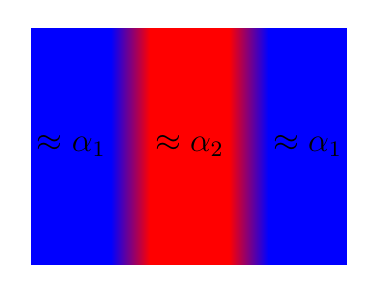
\begin{tikzpicture}
		\filldraw[fill=blue, draw=blue] (0,0) rectangle (1,3);
		\shade[left color=blue,right color=red] (1,0) rectangle (1.5,3);
		\filldraw[fill=red, draw=red] (1.5,0) rectangle (2.5,3);
		\shade[left color=red,right color=blue] (2.5,0) rectangle (3,3);
		\filldraw[fill=blue, draw=blue] (3,0) rectangle (4,3);
		
		\node at (0.5,1.5) {\large $\approx \alpha_{ 1 } $};
		\node at (2,1.5) {\large $\approx \alpha_{ 2 } $};
		\node at (3.5,1.5) {\large $\approx \alpha_{ 1 } $};
		
	\end{tikzpicture}
	
	\caption{$ \varepsilon > 0 $}
	\label{subfigure_epsilon}
	\end{subfigure}
	\hfill
	\begin{subfigure}[b]{0.3\linewidth}
		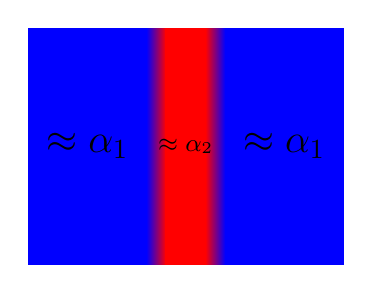
\begin{tikzpicture}
		\filldraw[fill=blue, draw=blue] (0,0) rectangle (1.5,3);
		\shade[left color=blue,right color=red] (1.5,0) rectangle (1.75,3);
		\filldraw[fill=red, draw=red] (1.75,0) rectangle (2.25,3);
		\shade[left color=red,right color=blue] (2.25,0) rectangle (2.5,3);
		\filldraw[fill=blue, draw=blue] (2.5,0) rectangle (4,3);
		
		\node at (0.75,1.5) {\Large $\approx \alpha_{ 1 } $};
		\node at (2,1.5) {\small $\approx \alpha_{ 2 } $};
		\node at (3.25,1.5) {\Large $\approx \alpha_{ 1 } $};
			
		\end{tikzpicture}
	
		\caption{$ \varepsilon > \varepsilon' >0 $}
		\label{subfigure_varepsilon_prime}
	\end{subfigure}
	\hfill
	\begin{subfigure}[b]{0.3\linewidth}
		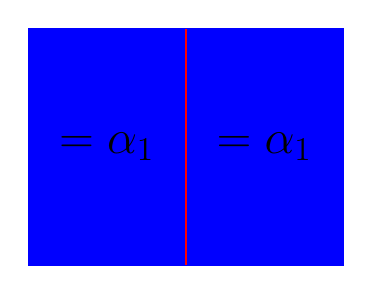
\begin{tikzpicture}
			\filldraw[fill=blue, draw=blue] (0,0) rectangle (4,3);
			\draw[red,thick](2,0)--(2,3);
			
			\node at (1,1.5) {\LARGE $= \alpha_{ 1 } $};
			\node at (3,1.5) {\LARGE $= \alpha_{ 1 } $};
			
		\end{tikzpicture}
		
		\caption{$ \varepsilon = 0 $}
		\label{subfigure_varepsilon_zero}
	\end{subfigure}

	\caption{Profile of the solution $u_{ \varepsilon } $ as $ \varepsilon $ 
	tends to zero.}
	\label{figure_interfaces_collapse}
\end{figure}

This leads us to the solution concept introduced by Hensel and Laux in 
\cite{hensel_laux_varifold_solution_concept_for_mean_curvature_flow}.
For the twophase case, the definition is as follows.

\begin{definition}[De Giorgi type varifold solutions for twophase mean 
curvature flow]
	Let $ \mu = \lm^{ 1 } \otimes ( \mu_{ t } )_{ t \in ( 0 , \infty ) } $ be a 
	family of oriented varifolds $ \mu_{ t } \in \mathcal{ M } \left( 
	\flattorus \times \mathbb{ S }^{ d - 1 } \right) $, $ t \in ( 0 , \infty ) 
	$, such that the map $ t \mapsto \int_{ \flattorus \times \mathbb{ S }^{ d 
	-1 } } \eta ( x , p , t ) \dd \mu_{ t } ( x , p ) $ is measurable for all 
	$ \eta \in \lp^{ 1 } \left( ( 0 , \infty ) ; \cont \left( \flattorus, 
	\mathbb{ S 
	}^{ d - 1 } \right) \right) $. 
	Consider also a family $ A = ( A_{ t } )_{ t \in ( 0 , \infty ) } $ of 
	subsets $ \flattorus $ with finite perimeter such that the associated 
	indicator function $ \chi ( x , t ) = \chi_{ A _{ t } } ( x ) $ satisfies 
	$ \chi \in \lp^{ \infty } \left( ( 0 , \infty ) ; \bv ( \flattorus ; \{ 0 , 
	1 \} ) \right) $.
	Let $ \sigma > 0 $ be a surface tension constant.
	
	Given an initial oriented varifold 
	$ \mu^{ 0 } \in \mathcal{ M } \left( \flattorus \times \mathbb{ S }^{ d - 1 
	} \right) $ and an initial phase indicator function $ \chi^{ 0 } \in \bv 
	\left( \flattorus ; \{ 0 , 1 \} \right)$, we call the pair $ ( \mu , \chi ) 
	$ a \emph{De Giorgi type varifold solution for twophase mean curvature flow 
	with initial data} $ ( \mu^{ 0 } , \chi^{ 0 } ) $ if the following holds.
	\begin{enumerate}
		\item (Existence of a normal speed)
		Writing $ \mu_{ t } = \omega_{ t } \otimes ( \lambda_{ x , t } )_{ x 
		\in \flattorus} $ for the disintegration of $ \mu_{ t } $, we require 
		the existence of some 
		$ V \in \lp^{ 2 } \left( ( 0 , \infty ) ; \lp^{ 2 } \left( \flattorus ; 
		\omega_{ t } \right) \right) $ encoding a normal speed in the sense of
		\begin{equation}
			\label{equation_varifold_velocity}
			\sigma
			\int
				\chi ( T , x ) \varphi ( T , x ) 
				-
				\chi^{ 0 } ( x ) \varphi (0,x)
			\dd{ x }
			=
			\sigma
			\int_{ 0 }^{ T }
				\int
					\chi
					\partial_{ t } \varphi 
				\dd{ x }
			\dd{ t }
			+
			\int_{ 0 }^{ T }
				\int
					V \varphi 
				\dd{ \omega_{ t } }
			\dd{ t }
		\end{equation}
		for almost every $ T \in ( 0 , \infty ) $ and all $ \varphi \in \cont_{ 
		\mathrm{c} }^{ \infty } \left( [ 0 , \infty ) \times \flattorus \right) 
		$.
		
		\item (Existence of a generalized mean curvature vector)
		We require the existence of some 
		$ H \in \lp^{ 2 } \left( 
			( 0 , \infty ) ; 
			\lp^{ 2 } \left(
				\flattorus , \omega_{ t } ; \mathbb{ R }^{ d }
			\right)
			\right) $
		encoding a generalized mean curvature vector by
		\begin{equation}
			\label{equation_varifold_mean_curvature}
			\int_{ 0 }^{ \infty }
				\int
					\inner*{ H }{ \xi }
				\dd{ \omega_{ t } }
			\dd{ t }
			=
			-
			\int_{ 0 }^{ \infty }
				\int_{ \flattorus \times \mathbb{ S }^{ d - 1 } }
					\inner*{ \xi }{ \mathrm{Id} - p \otimes p }
				\dd{ \mu_{ t } }
			\dd{ t }
		\end{equation}
		for all $ \xi \in \cont_{ \mathrm{c} }^{ \infty } \left( [ 0, \infty ) 
		\times \flattorus ; \mathbb{ R }^{ d } \right) $.
		
		\item (De Giorgi type optimal energy dissipation inequality)
		A sharp energy dissipation inequality holds in form of
		\begin{equation}
			\label{equation_varifold_de_giorgi_inequality}
			\omega_{ T } ( \flattorus )
			+
			\frac{ 1 }{ 2 }
			\int_{ 0 }^{ T }
				\int
					V^{ 2 }
					+
					\abs{ H }^{ 2 }
				\dd{ \omega_{ t } }
			\dd{ t }
			\leq
			\omega_{ 0 } ( \flattorus )
		\end{equation}
		for almost every $ T \in ( 0 , \infty ) $.
		
		\item (Compatibility)
		For almost every $ t \in ( 0 , \infty ) $ and all $ \xi \in \cont^{ 
		\infty } \left( \flattorus ; \mathbb{ R }^{ d } \right) $, it holds that
		\begin{equation}
			\label{equation_varifold_compatibility}
			\sigma
			\int
				\inner*{ \xi }
				{ \nabla \chi ( t , \cdot ) }
			=
			\int_{ \flattorus \times \mathbb{ S }^{ d - 1 } }
				\inner*{ \xi }{ p }
			\dd{ \mu_{ t } }.
		\end{equation}
	\end{enumerate}
\end{definition}

We firstly want to discuss this definition. In the setting of 
\Cref{de_giorgi_solution_to_mmcf} and in the twophase case, we can think of the 
oriented varifold $ \mu $ as the measure 
\begin{equation} 
	\label{equation_simple_varifold}
\mu =
\sigma \lm^{ 1 } |_{ 
( 0 , \infty ) } \otimes \abs{ \nabla \chi  ( t ) } 
\otimes \delta_{ \nu ( t , x ) }, 
\end{equation}
and therefore the measure $ \omega_{ t } $ 
becomes the energy measure $ \energy ( \chi ( t ) , \cdot ) $.
The advantage of this formulation is that our new energy measure $ \omega_{ t } 
$ is not restricted to only seeing the measure theoretic boundary of $ \chi $, 
but can actually capture phenomenons as described in 
\Cref{figure_interfaces_collapse}.
For example in such a scenario we would expect the measure $ \mu_{ t } $ to be 
defined by
\begin{equation}
	\label{equation_mu_in_figure}
	\mu_{ t } \coloneqq
	2 \hm^{ 1 } |_{ l } \otimes \frac{ 1 }{ 2 } \left( \delta_{ ( 1 , 0 ) } + 
\delta_{ ( - 1 , 0 ) }\right) ,
\end{equation}
where $ l $ is the red line to which the phase 
of $ \alpha_{ 2 } $ shrank down as $ \varepsilon $ approached zero. The factor 
2 comes from the fact that we obtain energy from both the collapsing interfaces.

The equation (\ref{equation_varifold_velocity}) for the  normal speed is simply 
motivated through 
the fundamental theorem of calculus. Assuming that everything is nice and 
smooth, we can compute that 
\begin{align*}
	\sigma \int
		\chi ( T , x ) \varphi ( T , x ) - \chi^{ 0 } ( x ) \varphi ( 0 , x )
	\dd{ x }
	& =
	\sigma \int_{ 0 }^{ T }
		\int
			\partial_{ t } \left(
				\chi ( t , x ) \varphi ( t , x )
			\right)
		\dd{ x }
	\dd{ t }
	\\
	&=
	\sigma \int_{ 0 }^{ T }
		\int
			\partial_{ t } \chi ( t , x ) \varphi ( t , x )
			\chi ( t , x ) \partial_{ t } \varphi ( t , x )
		\dd{ x }
	\dd{ t }
	\\
	& =
	\sigma \int_{ 0 }^{ T }
		\int
			\chi ( t , x )
			\partial_{ t } ( t , x )
		\dd{ x }
	\dd{ t }
	+
	\int_{ 0 }^{ T }
		\int
			V \varphi 
		\dd{ \omega_{ t} }
	\dd{ t },
\end{align*}
where for the last equality, we used $ \partial_{ t } \chi = V \abs{ \nabla 
\chi } \dd{ t } $ and $ \omega_{ t } = \sigma \abs{ \nabla \chi ( t ) } $.

The equation (\ref{equation_varifold_mean_curvature}) for the generalized mean 
curvature is also quite intuitive since 
assuming that the simple case of the varifold (\ref{equation_simple_varifold}) 
holds, we have that the right hand side of equation 
(\ref{equation_varifold_mean_curvature}) reads
\begin{equation*}
	\int_{ \flattorus \times \mathbb{ S }^{ d - 1 } }
		\inner*{ \xi }{ \mathrm{Id} - p \otimes p }
	\dd{ \omega_{ t } }
	=
	\sigma
	\int
		\inner*{ \xi }{\mathrm{Id} - \nu \otimes \nu }
	\abs{ \nabla \chi },
\end{equation*}
which is the standard distributional formulation for the mean curvature vector.

De Giorgis inequality (\ref{equation_varifold_de_giorgi_inequality}) is 
self-explanatory since $ \omega_{ t } $ is the energy measure. The 
compatibility condition is necessary to couple the evolving set $ A_{ t } $ to 
the varifold. Notice that in our above example (\ref{equation_mu_in_figure}), 
we have that even though the energy measure $ \omega_{ t } $ sees the red strip 
and the measure theoretic boundary of the corresponding indicator function does 
not, the term on the right hand side of (\ref{equation_varifold_compatibility}) 
is zero since
\begin{equation*}
	\int_{ \flattorus \times \mathbb{ S }^{ d - 1 } }
		\inner*{ \xi }{ p }
	\dd{ \mu_{ t } }
	=
	\int_{ l }
		\frac{ 1 }{ 2 }
		\inner*{ \xi }{ ( 1 , 0 ) + ( - 1 , 0 ) }
	\dd{ \hm^{ 1 } }
	= 
	0,
\end{equation*} 
and thus we have no problem.

For the multiphase case, we propose the following solution concept, which 
generalized 
\cite[Def.~2]{hensel_laux_varifold_solution_concept_for_mean_curvature_flow} to 
the case of arbitrary surface tensions.

\begin{definition}[De Giorgi type varifold solutions for multiphase mean 
curvature flow]
	\label{de_giorgi_varifold_solutions_for_mmcf}
	Let $ P \in \mathbb{ N }_{ \geq 2 } $ be the number of phases. For each 
	pair of phases $ ( i , j ) \in \{ 1 , \dotsc, P \} $, let 
	$ \mu^{ i j } = \lm^{ 1 }|_{ ( 0 , \infty ) } $ be a family of oriented 
	varifolds 
	$ \mu_{ t }^{ i j } \in \mathcal{ M } \left(
		\flattorus \times \mathbb{ S }^{ d - 1 }
	\right) $,
	$ t \in ( 0 , \infty ) $, such that the map 
	$ t \mapsto \int_{ \flattorus \times \mathbb{ S }^{ d - 1 } }
		\eta ( t , x , p )
	\dd{ \mu_{ t }^{ i j } ( x, p ) }$
	is measurable for all test functions 
	$ \eta \in \lp^{ 1 } \left(	
		( 0 , \infty ) ; \cont \left( \flattorus \times \mathbb{ S }^{ d- 1 } 
		\right) 
	\right) $.
	Define evolving oriented varifolds $ \mu^{ i } = \lm^{ 1 }|_{ ( 0 , \infty 
	) } \otimes ( \mu_{ t }^{ i } )_{ t \in ( 0 , \infty ) } $, $ i \in \{ 1, 
	\dotsc, P \} $ and $ \mu = \lm^{ 1 }|_{ ( 0 , \infty ) } \otimes ( \mu_{ t 
	} )_{ t \in ( 0 , \infty ) } $ by means of
	\begin{align*}
		\mu_{ t }^{ i }
		& \coloneqq
		2 \mu_{ t }^{ i , i }
		+
		\sum_{ j = 1 , j \neq i }^{ P }
			\mu_{ t }^{ i j },
		\\
		\mu_{ t }
		& \coloneqq
		\frac{ 1 }{ 2 }
		\sum_{ i = 1 }^{ P }
			\mu_{ t }^{ i }.
	\end{align*}
	The disintegration of $ \mu_{ t }^{ i j } $ is expressed in form of 
	$ \mu_{ t }^{ i j } = \omega_{ t }^{ i j } \otimes \left( \lambda _{ t , x 
	}^{ i j } \right)_{ x \in \flattorus } $ with expected value
	$ \langle \lambda_{ t , x }^{ i j } \rangle 
	\coloneqq
	\int_{ \mathbb{ S }^{ d - 1 } }
		p 
	\dd{ \lambda_{ t , x }^{ i j } ( p ) } $.
	Analagous expressions are introduced for the disintegrations of $ \mu_{ t 
	}^{ i } $ and $ \mu_{ t } $.
	
	Furthermore consider a family 
	$ A = \left( A^{ 1 } , \dotsc , A^{ P } \right) $ 
	such that for each phase $ 1 \leq i \leq P $, we have a family
	$ A^{ i } = ( A^{ i } ( t ) )_{ t \in ( 0 , \infty ) } $ of subsets of $ 
	\flattorus $ with finite perimeter. We also require 
	$ \left( A^{ 1 } ( t ) , \dotsc, A^{ P } ( t ) \right) $
	to be a partition of $ \flattorus $ for all $ t \in ( 0 , \infty ) $ and 
	that for each $ 1 \leq i \leq P $, the associated indicator function 
	satisfies 
	$ \chi^{ i } \in \lp^{ \infty } \left(
		( 0 , \infty ) ;
		\bv \left( \flattorus ; \{ 0 , 1 \} \right)
	\right) $.
	We shortly write $ \chi = \left( \chi^{ 1 } , \dotsc, \chi^{ P } \right) $.
	
	Given initial data 
	$ (
		( \mu_{ 0 }^{ i j } )_{ 1 \leq i , j \leq P },
		( \chi^{ i}_{ 0 } )_{ 1 \leq i \leq P}
	) $
	of the above form and a $ P \times P $ matrix of surface tensions $ \sigma 
	$ such that $ \sigma_{ i i }=0 $ and $ \sigma_{ i j } > 0 $ for $ i \neq j 
	$, we call the pair $ \left( \mu , \chi \right) $ a
	\emph{De Giorgi type varifold solution for multiphase mean curvature flow 
	with initial data} $ ( \mu_{ 0 } , \chi_{ 0 } ) $ \emph{and surface 
	tensions} $ \sigma $ if the following requirements hold true.
	\begin{enumerate}
		\item (Existence of normal speeds)
		For each phase $ 1 \leq i \leq P $, there exists a normal speed
		$ V^{ i } \in \lp^{ 2 } \left(
			( 0 , \infty ) ;
			\lp^{ 2 } \left( \flattorus , \omega_{ t }^{ i } \right)
		\right) $ in the sense that
		\begin{equation}
			\label{equation_varifold_velocity_multiphase}
			\int
				\chi^{ i } ( T, x ) \varphi ( T, x ) 
				-
				\chi^{ i }_{ 0 } ( x ) \varphi ( 0 , x )
			\dd{ x }
			=
			\int_{ 0 }^{ T }
				\int
					\chi^{ i }
					\partial_{ t } \varphi
				\dd{ x }
			\dd{ t }
			+
			\sum_{ j =1, \j \neq i  }^{ P }
				\frac{ 1 }{ \sigma_{ i j } }
				\int_{ 0 }^{ T }
					\int
						V^{ i }
						\varphi
					\dd{ \omega_{ t }^{ i j } }
				\dd{ t }
		\end{equation}
		for almost every $ T \in ( 0 , \infty ) $ and all $ \varphi \in \cont_{ 
		\mathrm{c} }^{ \infty } \left( [ 0 , \infty ) \times \flattorus\right) 
		$.
	\end{enumerate}

	\item (Existence of a generalized mean curvature vector)
	There exists a generalized mean curvature vector 
	$ H \in \lp^{ 2 } \left(
		( 0 , \infty ) ;
		\lp^{ 2 } \left( \flattorus , \omega_{ t } ; \mathbb{ R }^{ d } \right)
	\right) $
	in the sense that
	\begin{equation}
		\label{equation_varifold_mean_curvature_multiphase}
		\int_{ 0 }^{ T }
			\int
				\inner*{ H }{ \xi }
			\dd{ \omega_{ t } }
		\dd{ t }
		=
		-
		\int_{ 0 }^{ T }
			\int_{ \flattorus \times \mathbb{ S }^{ d - 1 } }
				\inner*{ \diff \xi }
				{ \mathrm{Id} - p \otimes p }
			\dd{ \mu_{ t } }
		\dd{ t }
	\end{equation}
	holds for almost every $ T \in ( 0 , \infty ) $ and all $ \xi \in \cont_{ 
	\mathrm{c} }^{ \infty } \left( [ 0 , \infty ) \times \flattorus ; \mathbb{ 
	R }^{ d } \right) $.
	
	\item (De Giorgi type optimal energy dissipation inequality)
	A sharp energy dissipation inequality holds in form of
	\begin{equation}
		\label{equation_varifold_energy_dissipation_inequality}
		\omega_{ T } ( \flattorus )
		+
		\frac{ 1 }{ 2 }
		\sum_{ i = 1 }^{ P }
			\int_{ 0 }^{ T }
				\int
					( V^{ i } )^{ 2 }
					\frac{ 1 }{ 2 }
				\dd{ \omega_{ t }^{ i } }
			\dd{ t }
		+
		\frac{ 1 }{ 2 }
		\int_{ 0 }^{ T }
			\int
				\abs{ H }^{ 2 }
			\dd{ \omega_{ t } }
		\dd{ t }
		\leq
		\omega_{ 0 } ( \flattorus )
	\end{equation}
	for almost every $ T \in ( 0 , \infty ) $.
	
	\item (Compatibility conditions)
	For all $ 1 \leq i , j \leq P $ with $ i \neq j $, we require 
	\begin{equation}
		\label{varifold_symmetry_of_energy_measures}
		\omega_{ t }^{ i j }
		=
		\omega_{ t }^{ j i } 
	\end{equation}
	for almost every $ t \in ( 0 , \infty ) $ and
	\begin{align}
		\label{varifold_symmetry_expectations}
		\langle \lambda_{ t, x  }^{ i j } \rangle
		&= 
		- \langle \lambda_{ t, x  }^{ j i } \rangle,
		\\
		\label{varifold_expecation_of_ii_zero}
		\langle \lambda_{ t , x }^{ i i } \rangle
		&= 
		0,
		\\
		\label{varifold_symmetry_velocities}
		V^{ i } ( t, x ) 
		&= 
		- V^{ j } ( t, x ),
		\\
		\label{varifold_mean_curvature_points_in_normal_direction}
		\abs{ \langle \lambda_{ t , x }^{ i j } \rangle }^{ 2 }
		H ( t, x )
		& =
		\inner*{ H( t , x ) }{ \langle \lambda_{ t , x }^{ i j } \rangle }
		\langle \lambda_{ t , x }^{ i j } \rangle
	\end{align}
	for almost every $ t \in ( 0 , \infty ) $ and $ \omega_{ t }^{ i j } $ 
	almost every $ x \in \flattorus $. Finally for all $ 1 \leq i \leq P $, we 
	have
	\begin{equation}
		\label{varifold_compatibility_condition_multiphase}
		\int
			\inner*{ \xi }{ \dd{ \nabla \chi^{ i } ( t , \cdot ) } }
		=
		\sum_{ j = 1 , j \neq i }^{ P }
			\frac{ 1 }{ \sigma_{ i j } }
			\int_{ \flattorus \times \mathbb{ S }^{ d - 1 } }
				\inner*{ \xi }{ p }
			\dd{ \mu_{ t }^{ i j } }
	\end{equation}
	for almost every $ t \in ( 0 , \infty ) $ and every $ \xi \in \cont^{ 
	\infty } \left( \flattorus ; \mathbb{ R }^{ d } \right) $.
\end{definition}

As before, we first want to motivate this definition. In the simplest case, we 
can think of the varifold $ \mu_{ t }^{ i j } $ for $ i \neq j $ as
\begin{equation}
	\label{varifold_simplest_case_mutliphase}
	\mu_{ t }^{ i j }
	=
	\sigma_{ i j }
	\dd{ \hm^{ d - 1 }|_{ \Sigma_{ i j } } } 
	\otimes
	( \delta_{ nu_{ i } } )_{ x \in \flattorus }.
\end{equation}
Under the assumption of energy convergence, we expect that $ \mu_{ t }^{ i i } 
= 0 $. But if approximate interfaces collapse as in 
\Cref{figure_interfaces_collapse}, then this is exactly captured by the 
varifold $ \mu_{ t }^{ i i }$, which, as in the twophase case, will be 
described by
\begin{equation}
	\label{varifold_when_interfaces_collapse}
	\mu_{ t }^{ i i}
	\coloneqq
	2 \hm^{ 1 } |_{ l }
	\otimes
	\frac{ 1 }{ 2 } 
	\left( \delta_{ ( 1 , 0 ) } + \delta_{ ( - 1 , 0 ) } \right).
\end{equation}
BIN MIR TATSÄCHLICH NICHT SICHER, OB DAS STIMMT; MIT TIM BESPRECHEN.
